\question{10.5}{
    Bij een onderzoek naar het gebruik van internet werden de respondenten onderverdeeld naar leeftijd en het wel of niet werken met internet.
    Voor $400$ respondenten leverde dit de volgende tabel:

    \begin{center}
        \begin{tabular}{cccc}
            \multicolumn{4}{l}{Internetgebruik} \\
            \toprule
                {\bfseries Leeftijd} & {\bfseries Wel internet} & {\bfseries Geen internet} & {\bfseries Totaal} \\
            \cmidrule{1-1} \cmidrule{2-2} \cmidrule{3-3} \cmidrule{4-4}
                Tot en met $44$ jaar & $143$ & $77$ & $220$ \\
                $45$ jaar en ouder & $97$ & $83$ & $180$ \\
            \cmidrule{1-1} \cmidrule{2-2} \cmidrule{3-3} \cmidrule{4-4}
                Totaal & $240$ & $160$ & $400$ \\
            \bottomrule
        \end{tabular}
    \end{center}
}
\begin{enumerate}[label=(\alph*)]
    \item De vraag is of deze indelingen onafhankelijk zijn.
    Bereken de \emph{expected}-tabel en voer de chikwadraattoets uit met behulp van de tabel (kies $\alpha=0,01$).
    \answer{
        Bij een chikwadraattoets voor onafhankelijkheid beginnen we met het defini\"eren van de nulhypothese $H_0$ en de alternatieve hypothese $H_1$.
        \begin{align*}
            H_0: &\quad \text{``leeftijd'' en ``internetgebruik'' zijn onafhankelijk van elkaar.} \\
            H_1: &\quad \text{``leeftijd'' en ``internetgebruik'' zijn  afhankelijk van elkaar.}
        \end{align*}
        Het significantieniveau $\alpha=0,01$ is gegeven in de opdracht, net als de geobserveerde data.
        Om de toetsingsgrootheid $X^2$ te kunnen bepalen, moeten we eerst de \emph{expected}-tabel berekenen.
        Hiervoor starten we vanuit een lege tabel waarin alleen de totalen (van de rijen en kolommen respectievelijk) gegeven zijn:
        
        \begin{center}
            \renewcommand{\arraystretch}{1.25}
            \begin{tabular}{cccc}
                \multicolumn{4}{l}{Internetgebruik} \\
                \toprule
                    {\bfseries Leeftijd} & {\bfseries Wel internet} & {\bfseries Geen internet} & {\bfseries Totaal} \\
                \cmidrule{1-1} \cmidrule{2-2} \cmidrule{3-3} \cmidrule{4-4}
                    Tot en met $44$ jaar & $$ & $$ & $220$ \\
                    $45$ jaar en ouder & $$ & $$ & $180$ \\
                \cmidrule{1-1} \cmidrule{2-2} \cmidrule{3-3} \cmidrule{4-4}
                    Totaal & $240$ & $160$ & $400$ \\
                \bottomrule
            \end{tabular}
        \end{center}

        Voor iedere cel in de tabel bepalen we de expected frequentie met de formule:

        \[
            E_{ij} = \frac{\text{rijtotaal}_{i} \cdot \text{kolomtotaal}_{j}}{\text{totaal}}
        \]

        Dit geeft de volgende \emph{expected}-tabel:

        \begin{center}
            \renewcommand{\arraystretch}{1.5}
            \begin{tabular}{cccc}
                \multicolumn{4}{l}{Internetgebruik} \\
                \toprule
                    {\bfseries Leeftijd} & {\bfseries Wel internet} & {\bfseries Geen internet} & {\bfseries Totaal} \\
                \cmidrule{1-1} \cmidrule{2-2} \cmidrule{3-3} \cmidrule{4-4}
                    Tot en met $44$ jaar & $\frac{220\cdot 240}{400}=132$ & $\frac{220\cdot 160}{400}=88$ & $220$ \\
                    $45$ jaar en ouder & $\frac{180\cdot 240}{400}=108$ & $\frac{180\cdot 160}{400}=72$ & $180$ \\
                \cmidrule{1-1} \cmidrule{2-2} \cmidrule{3-3} \cmidrule{4-4}
                    Totaal & $240$ & $160$ & $400$ \\
                \bottomrule
            \end{tabular}
        \end{center}

        De toetsingsgrootheid $X^2$ bepalen we aan de hand van de volgende formule:

        \begin{align*}
            X^2  &= \sum_{i,j} \frac{(O_{ij} - E_{ij})^2}{E_{ij}},
        \end{align*}

        waarbij $i = 1,2$ de index van de rij is, en $j = 1,2$ de index van de kolom is.
        Dit geeft in dit specifieke geval een geobserveerde toetsingsgrootheid 
        
        \begin{align*}
            \chi^2  &= \sum_{i,j} \frac{(O_{ij} - E_{ij})^2}{E_{ij}} \\
                    &=\frac{(O_{11} - E_{11})^2}{E_{11}} + \frac{(O_{12} - E_{12})^2}{E_{12}} + \frac{(O_{21} - E_{21})^2}{E_{21}} + \frac{(O_{22} - E_{22})^2}{E_{22}} \\
                    &= \frac{(143 - 132)^2}{132} + \frac{(77 - 88)^2}{88} + \frac{(97 - 108)^2}{108} + \frac{(83-72)^2}{72}\\
                    &\approx 4,6402
        \end{align*}

        Onder de nulhypothese volgt de toetsingsgrootheid $X$ een chikwadraatverdeling met
        \[
            \text{df} = (\#\text{rijen}-1) \cdot (\#\text{kolommen}-1) = (2-1)\cdot(2-1) = 1
        \]
        vrijheidsgraad.
        De $p$-waarde (rechteroverschrijdingskans) die hoort bij deze geobserveerde toetsingsgrootheid $\chi^2$ is gelijk aan
        \begin{align*}
            p   &= P(X^2 \ge \chi^2) \\
                &= \chi^2\text{cdf}(\text{lower}=\chi^2\approx4,6402; \text{upper}=10^{10}; \text{df}=1) \\
                &\approx 0,0312
        \end{align*}

        Aangezien de $p$-waarde groter is dan het significantieniveau $\alpha=0,01$, wordt $H_0$ niet verworpen.
        Er is onvoldoende bewijs om de hypothese te verwerpen dat de twee nominale variabelen ``leeftijd'' en ``internetgebruik'' onafhankelijk zijn van elkaar.
        
        \begin{center}
            \resizebox{0.9\textwidth}{!}{
                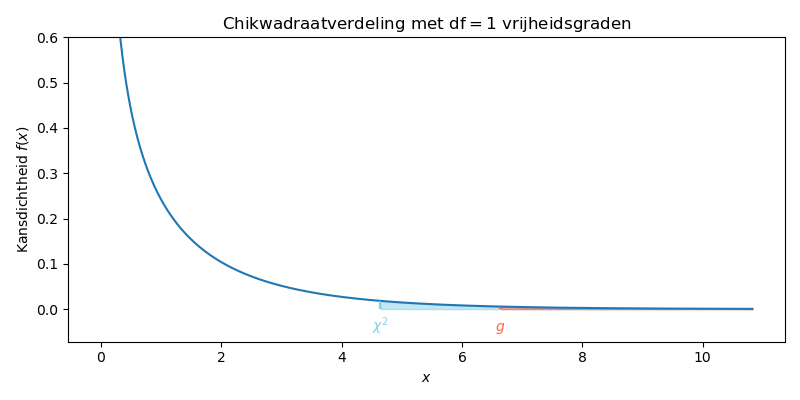
\includegraphics{opg_10.5.png}
            }
        \end{center}
    }
\end{enumerate}